% Provenance (never printed): see sources/outline_sources.md (Year 2: monsoons; El Niño--Southern
% Oscillation; the North Atlantic Oscillation; ocean--atmosphere coupling). Definitions after the
% IPCC AR6 glossary, the NOAA CPC ENSO FAQ and NAO pages, the NWS glossary and the IMD monsoon
% FAQ; indices from the CPC data files (data/derived/bachelor-2-{oni,oni-table,roni,nino34,nao});
% figures from figdata/bachelor-2/climvar.py; values of the examples, exercises and problem
% computed in the Book 4 scratch calculator calc/ch23.py.
\chapter{Climate Variability}\label{ch:b2:climate-variability}

In September 2026 the sea surface in the central equatorial Pacific averaged \qty{29.27}{\celsius},
where the usual September value is \qty{26.71}{\celsius}; farther east, parts of the ocean were
more than \qty{4}{\celsius} warmer than usual, and forecasters put at more than four in five the
chance that the event would, by the end of the year, exceed every El~Niño since 1950. The earlier
record events, in 1982, 1997 and 2015, bleached and killed corals, set tropical forests on fire
and brought heat waves; the anchovy catch of Peru falls steeply when such warm water lingers. The
ocean and the atmosphere of the tropical Pacific had swung, as they do every few years, and the
swing reached far beyond the Pacific. This
chapter describes such swings of the climate, the \omterm{def:b2:climate-variability:monsoon}{monsoons}, El~Niño and La~Niña, the \omterm{def:b2:climate-variability:nao}{North
Atlantic Oscillation}, and what makes the ocean their memory.
% ledger: data:b4-nino34, cpc:edd-2026-10, thirumalai24:bjerknes, cheung26:peru

\begin{recall}
\textbf{From the school volumes}: weather and climate; the temperature anomaly; the mixed layer,
the thermocline and upwelling; the climate feedback. \textbf{From the Year 1 volume}: the Hadley
cells, the trade winds, the intertropical convergence zone and its seasonal migration, the Walker
circulation, coastal upwelling. \textbf{From \cref{ch:b2:weather-systems}}: the jet stream,
\omterm{def:b2:weather-systems:rossby}{Rossby waves}, \omterm{def:b2:weather-systems:cyclones}{extratropical cyclones} and blocking. \textbf{From the physics books}: heat capacity
and the first law of thermodynamics.
\end{recall}

\section{Variability and its measures}\label{sec:b2:climate-variability:measures}

Weather changes from day to day; climate, the statistics of weather, changes too, from one season
or one year to the next, even when nothing outside the climate system changes. Some of that
variability is noise, but much of it is organised into a few patterns that recur, with their own
geography and their own time scales.

\begin{definition}[Mode of climate variability; climate index; climatology]\label{def:b2:climate-variability:modes}
A \emph{mode of climate variability}\index{mode of climate variability} is a recurrent pattern of
natural variability of the climate system, with its own spatial pattern, seasonality and time
scales, arising from the dynamics of the atmosphere or from the coupling of the ocean and the
atmosphere. A \emph{climate index}\index{climate index} is a time series built from climate
variables that summarises the state of such a pattern, for example the difference of sea-level
pressure between Iceland and the Azores. The \emph{climatology}\index{climatology} of a variable
is its mean over a reference period, computed for each calendar month or season; the standard
reference period is 30 years long, currently 1991--2020.
\end{definition}
% ledger: ipccgl:modes, ipccgl:index, wmo:normal-30yr

Many modes are driven by processes internal to the climate system: they are part of its
internal variability. Because they recur with their own time scales, they are a source of
predictability beyond the reach of weather forecasts, from weeks to decades. Indices make them
measurable. An index is computed from anomalies, as in the school volumes, and
smoothed.
% ledger: ipccgl:modes

\begin{method}[From observations to an index]\label{met:b2:climate-variability:index}
\begin{enumerate}
  \item Compute the \omterm{def:b2:climate-variability:modes}{climatology}: the mean of the variable for each calendar month over the
        reference period.
  \item Subtract it: the anomaly of each month is its value minus the \omterm{def:b2:climate-variability:modes}{climatology} of that month.
        The seasonal cycle disappears; what is left is the variability.
  \item Smooth the anomalies with a running mean, the mean of $n$ consecutive values centred on
        each month, to remove the fluctuations shorter than the pattern of interest.
  \item If the index is to be compared with others, divide by its standard deviation: the index
        is then standardised, in units of standard deviations.
\end{enumerate}
\end{method}

\begin{example}[An anomaly]\label{ex:b2:climate-variability:anomaly}
The mean sea-surface temperature of the central equatorial Pacific between \ang{5} N and
\ang{5} S, \ang{170} W and \ang{120} W was \qty{29.27}{\celsius} in September 2026. Its September
\omterm{def:b2:climate-variability:modes}{climatology} is \qty{26.71}{\celsius}, so the anomaly was $29.27 - 26.71 = \qty{2.56}{\celsius}$.
In September 1997 the same ocean was at \qty{28.79}{\celsius} against \qty{26.73}{\celsius}, an
anomaly of \qty{2.06}{\celsius}. The two climatologies differ slightly because the reference
period is moved every five years: the ocean itself has warmed.
% ledger: data:b4-nino34, cpc:oni-def
\end{example}

\section{Monsoons}\label{sec:b2:climate-variability:monsoons}

\begin{definition}[Monsoon]\label{def:b2:climate-variability:monsoon}
A \emph{monsoon}\index{monsoon} is a thermally driven wind, arising from the different heating of
a land mass and the adjacent ocean, that reverses its direction with the seasons, together with
the seasonal reversal of rainfall it brings.
\end{definition}
% ledger: nws4:monsoon, ipccgl:monsoon

On land the heat of the summer Sun stays in a thin layer near the surface, while the sea mixes
the same heat down through its mixed layer, tens of metres deep, and warms far less. The air over
the land warms more, its pressure at the surface falls, and moist air flows in from the sea, rises, cools and
rains; aloft the air returns seaward. In winter the land is the colder surface and the circulation
reverses. Taken together, the \omterm{def:b2:climate-variability:monsoon}{monsoons} of the planet form a single global pattern that dominates the yearly
cycle of tropical and subtropical rain; its domain is defined as the regions where the mean rain
of the local summer exceeds that of the winter by more than \qty{2.5}{mm} a day.
% ledger: nws4:monsoon, ipccgl:monsoon

\begin{omfigure}
\centering
\begin{tikzpicture}[font=\scriptsize, >=Stealth]
\foreach \col/\title in {0/{a\enspace summer}, 7.2/{b\enspace winter}} {
  \begin{scope}[shift={(\col,0)}]
  \node[anchor=south west] at (0,3.0) {\textbf{\title}};
  \fill[ocBlue!18] (0,0) rectangle (3,0.35);
  \fill[brown!35] (3,0) -- (6.4,0) -- (6.4,0.5) -- (3,0.35) -- cycle;
  \node at (1.5,0.17) {sea};
  \node at (4.7,0.2) {land};
  \end{scope}
}
% summer: low over the land, inflow from the sea, rising air and rain
\node[font=\small\bfseries, ocBlue] at (0.45,0.62) {H};
\node[font=\small\bfseries, ocRed] at (4.8,0.78) {L};
\node[ocRed, anchor=west] at (5.35,0.78) {hot};
\draw[->, thick] (1.0,0.98) -- (4.2,1.02);
\node at (2.4,0.66) {moist air from the sea};
\draw[->, thick] (4.8,1.15) -- (4.8,2.55);
\draw[->, thick] (4.45,2.8) -- (1.75,2.8);
\draw[->, thick] (1.4,2.6) -- (1.4,1.25);
\fill[black!15, draw=black!40] (4.0,1.9) .. controls (4.0,2.55) and (5.6,2.55) .. (5.6,1.9) -- cycle;
\foreach \x in {4.25,4.5,5.1,5.35} {\draw[ocBlue, dashed] (\x,1.85) -- (\x-0.1,1.2);}
\node[anchor=west] at (5.65,2.1) {rain};
% winter: high over the land, dry outflow to the sea
\begin{scope}[shift={(7.2,0)}]
\node[font=\small\bfseries, ocRed] at (0.45,0.62) {L};
\node[font=\small\bfseries, ocBlue] at (4.8,0.78) {H};
\node[ocBlue, anchor=west] at (5.35,0.78) {cold};
\draw[->, thick] (4.2,1.02) -- (1.0,0.98);
\node at (2.4,0.66) {dry air from the land};
\draw[->, thick] (1.4,1.25) -- (1.4,2.6);
\draw[->, thick] (1.75,2.8) -- (4.45,2.8);
\draw[->, thick] (4.8,2.55) -- (4.8,1.15);
\end{scope}
\end{tikzpicture}
\par\smallskip{\small The \omterm{def:b2:climate-variability:monsoon}{monsoon} as a land--sea circulation (schematic section, not to scale): in
summer the land is the warmer surface, with low pressure at the ground, inflow of moist air from
the sea, rising air and rain; in winter the circulation reverses and the land wind is dry.}
\end{omfigure}
% ledger: nws4:monsoon, imd:heat-low

The \omterm{def:b2:climate-variability:monsoon}{monsoon} of South and South-East Asia starts in late May or early June, progresses
north-eastward and ends in late September or early October. Before it, the lands around the
Arabian Sea heat up: in June the surface sends about \qty{160}{W/m^2} of heat into the air over
the arid north-west of India, Pakistan and the Middle East, and a shallow heat low forms there,
reaching only to about \qty{1.5}{km}, with little rain; a weak heat low, as in the drought year
1987, means a weak pull on the moist air of the ocean. From it an elongated trough of low pressure, the \omterm{def:b2:climate-variability:monsoon}{monsoon}
trough, runs to the head of the Bay of Bengal; its north--south oscillations bring the active
spells and the breaks of the season. Over India as a whole the rain of June to September averages
\qty{88}{cm}, with a standard deviation of \qty{9}{cm}, about \qty{10}{\percent}: a season within
\qty{10}{\percent} of the long-period average is called normal. On the Kerala coast, where the
national weather service declares the onset of the \omterm{def:b2:climate-variability:monsoon}{monsoon} from the rainfall of fourteen stations,
the winds and the satellite-measured outgoing infrared radiation, the average rainfall is
\qty{556}{mm} in June and \qty{659}{mm} in July.
% ledger: ipccgl:monsoon, imd:heat-low, imd:lpa, imd:onset

The West African \omterm{def:b2:climate-variability:monsoon}{monsoon} brings moist south-westerly winds from the Gulf of Guinea, progressing
northward from May to September; its rain peaks near \ang{12} N in late August and September and
retreats from October.
% ledger: ipccgl:monsoon

A \omterm{def:b2:climate-variability:monsoon}{monsoon} is regular in its timing, irregular in its amount, and the year-to-year swings of the
tropical Pacific are among the causes. El~Niño years tend to leave India short of rain: the
droughts of 1904, 1972 and 1987 came with El~Niño. The link is not certain: in 1997 a strong
El~Niño coincided with a positive phase of the Indian Ocean Dipole, a mode met below, and India
had a near-normal \omterm{def:b2:climate-variability:monsoon}{monsoon}.
% ledger: narang24:enso-monsoon, ipccgl:other-modes

\section{El Niño and the Southern Oscillation}\label{sec:b2:climate-variability:enso}

The Year~1 volume described the Walker circulation: air rising over the warm western Pacific,
flowing east aloft, sinking over the cool eastern Pacific and returning west with the trade
winds. In the ocean below, the trade winds pile warm water in the west, where the thermocline is
deep, and draw cold water up along the equator in the east, where it is shallow. This state is not
fixed.

\begin{definition}[El Niño--Southern Oscillation; El Niño; La Niña; Southern Oscillation]\label{def:b2:climate-variability:enso}
The \emph{El Niño--Southern Oscillation}\index{El Niño--Southern Oscillation} (ENSO) is the
coupled ocean--atmosphere mode of the tropical Pacific: coherent year-to-year variations of the
sea-surface temperature, the convective rainfall, the surface pressure and the circulation along
the equatorial Pacific, with preferred time scales of two to about seven years. \emph{El
Niño}\index{El Niño} is its warm phase, a warming of the sea surface of the central and
east-central equatorial Pacific; \emph{La Niña}\index{La Niña} is its cold phase, a cooling of the
same region. The \emph{Southern Oscillation}\index{Southern Oscillation} is its atmospheric part,
a see-saw of surface pressure between the western and the eastern tropical Pacific: during El~Niño
the pressure is higher than average over Indonesia and the western Pacific and lower over the
eastern Pacific, and the reverse during La~Niña.
\end{definition}
% ledger: cpc:enso-faq, cpc:enso-faq-so, ipccgl:enso

During El~Niño, the easterly trade winds weaken along the equator, and in the west the
low-level winds may even blow from the west; the warm water of the west spreads east, and the deep
convection and its rain follow it, leaving Indonesia and northern Australia drier. The sea surface
of the east-central Pacific is typically \qtyrange{1.5}{2.5}{\celsius} warmer than average, and
the thermocline there lies at \qtyrange{150}{175}{m}, deeper than usual. During La~Niña the trade
winds strengthen across the whole basin, the sea surface is \qtyrange{1}{2}{\celsius} colder than
average, and the thermocline in the east rises to \qtyrange{50}{100}{m}. The Walker circulation
weakens during El~Niño and strengthens during La~Niña. Episodes typically recur every three to
five years, at intervals that have ranged from two to seven; an El~Niño typically lasts nine to
twelve months, a La~Niña one to three years. Both tend to develop between March and June, to
peak between December and April and to weaken between May and July; their effects are strongest
from December to April, when the equatorial sea surface is warmest.
% ledger: cpc:enso-faq-features, cpc:enso-faq-timing

\begin{omfigure}
\centering
\begin{tikzpicture}[font=\scriptsize, >=Stealth, x=1cm, y=0.8cm]
\foreach \row/\title/\tw/\te/\rx/\cwidth in {
    0/{a\enspace neutral}/1.15/0.35/1.6/1.0,
    -4.6/{b\enspace El Niño}/0.95/0.85/5.6/1.4,
    -9.2/{c\enspace La Niña}/1.3/0.18/1.0/0.8} {
  \begin{scope}[shift={(0,\row)}]
  \node[anchor=south west] at (0,2.55) {\textbf{\title}};
  % ocean: warm layer above the thermocline
  \fill[ocBlue!20] (0,-1.5) rectangle (11,0);
  \fill[omWarm!25] (0,0) -- (0,-\tw) .. controls (4,-\tw) and (7,-\te) .. (11,-\te) -- (11,0) -- cycle;
  \draw[thick, ocBlue!70!black] (0,-\tw) .. controls (4,-\tw) and (7,-\te) .. (11,-\te);
  \draw (0,0) -- (11,0);
  % convection and Walker cell
  \fill[black!15, draw=black!40] ({\rx-\cwidth/2},0.5) .. controls ({\rx-\cwidth/2},2.1) and ({\rx+\cwidth/2},2.1) .. ({\rx+\cwidth/2},0.5) -- cycle;
  \draw[->, thick] (\rx,0.55) -- (\rx,2.15);
  \draw[->, thick] ({\rx+0.4},2.3) -- (9.6,2.3);
  \draw[->, thick] (10.0,2.1) -- (10.0,0.5);
  \draw[->, thick] (9.6,0.3) -- ({\rx+0.7},0.3);
  \end{scope}
}
\node[anchor=west] at (2.3,1.4) {rising air, rain};
\node[anchor=east] at (9.9,1.4) {sinking air};
\node at (6.0,0.55) {trade winds};
\node[anchor=west, ocBlue!70!black] at (7.6,-0.95) {thermocline};
\node[anchor=east] at (4.8,-4.6+1.4) {rain moves east};
\node at (8.2,-4.6+0.55) {weak trade winds};
\node at (6.0,-9.2+0.55) {strong trade winds};
\node[ocBlue!70!black, align=center] at (9.6,-9.2-0.8) {cold water\\near the surface};
\node[anchor=north west] at (0,-9.2-1.55) {west (Indonesia)};
\node[anchor=north east] at (11,-9.2-1.55) {east (South America)};
\end{tikzpicture}
\par\smallskip{\small The equatorial Pacific along the equator in the three phases of ENSO
(schematic, not to scale): the Walker circulation above, the warm upper layer and the
thermocline below. During El~Niño the trade winds weaken, the warm water and the rain spread east
and the thermocline in the east deepens to \qtyrange{150}{175}{m}; during La~Niña the trades
strengthen and the thermocline in the east rises to \qtyrange{50}{100}{m}.}
\end{omfigure}
% ledger: cpc:enso-faq-features, climategov:walker

The names come from different centuries and different sciences. Fishermen of the coast of
South America noticed a warming of their coastal waters around Christmas that disrupted the
fishery, and called it El~Niño, the boy child. Sir Gilbert Walker discovered the \omterm{def:b2:climate-variability:enso}{Southern
Oscillation} in the atmosphere, without linking it to the ocean. Only in the late 1960s did Jacob Bjerknes and others see that the
two were one phenomenon. The terms La~Niña and neutral gained prominence in the 1980s.
% ledger: climategov:enso-history, ipccgl:enso

\begin{history}[The boy child of the fishermen]
\begin{minipage}[t]{0.54\linewidth}\vspace{0pt}
Off the dry coast of Peru, the cold water that the winds draw up along the shore is rich in
nutrients and feeds a productive fishery. Its fishermen knew a warming that came around
Christmas, when the fish became scarce, and gave it the name of the child of the season. The
anchovy catch of Peru still follows ENSO: in a recent analysis, prolonged high temperature
anomalies made an extremely low catch more than nine times likelier, with a median fall of the
catch of about \qty{60}{\percent}; the strong El~Niño of 1997--98 stands out in the record.
\end{minipage}\hfill
\begin{minipage}[t]{0.42\linewidth}\vspace{0pt}
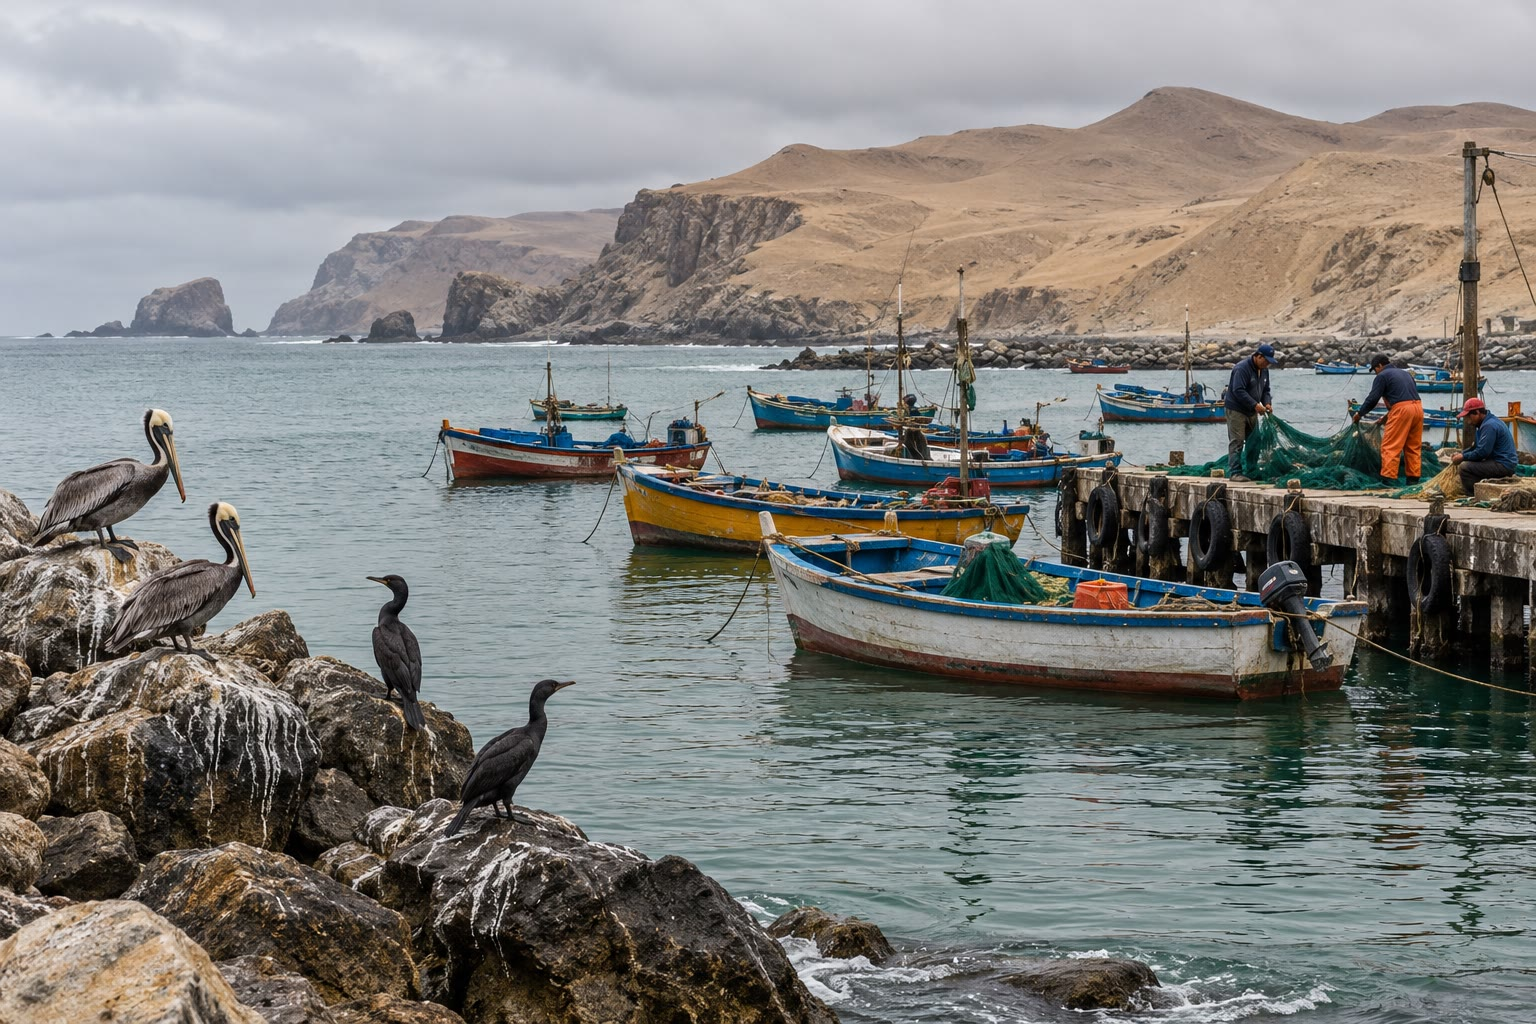
\includegraphics[width=\linewidth]{images/book4/ai/b2-fishing-harbour.jpg}

{\scriptsize Fishing boats in a harbour of a desert coast with cold upwelling water
(AI-generated illustration).}
\end{minipage}
% ledger: climategov:enso-history, cheung26:peru, stewart:upwelling
\end{history}

Why does the system swing at all? Because the ocean and the atmosphere of the equatorial Pacific
reinforce each other's anomalies.

\begin{definition}[Bjerknes feedback]\label{def:b2:climate-variability:bjerknes}
The \emph{Bjerknes feedback}\index{Bjerknes feedback} is the positive feedback between the
sea-surface temperature, the winds and the ocean currents of the equatorial Pacific: a warming of
the east weakens the east--west contrast of temperature and pressure, hence the trade winds;
weaker trade winds let the warm water of the west spread east and bring up less cold water in the
east, which warms the east further. The same loop amplifies a cooling.
\end{definition}
% ledger: thirumalai24:bjerknes, cpc:enso-faq-timing

\begin{omfigure}
\centering
\begin{tikzpicture}[font=\small, >=Stealth, box/.style={draw, rounded corners=2pt, fill=omDef!8,
  align=center, text width=4.3cm, minimum height=1.05cm, inner sep=3pt}]
\node[box] (a) at (0,2) {eastern equatorial Pacific\\warmer than usual};
\node[box] (b) at (6.2,2) {smaller east--west contrast\\of temperature and pressure};
\node[box] (c) at (6.2,0) {weaker trade winds};
\node[box] (d) at (0,0) {warm water spreads east,\\less cold water brought up};
\draw[->, very thick, ocRed] (a) -- (b);
\draw[->, very thick, ocRed] (b) -- (c);
\draw[->, very thick, ocRed] (c) -- (d);
\draw[->, very thick, ocRed] (d) -- (a);
\node[ocRed, font=\bfseries] at (3.1,1) {$+$};
\end{tikzpicture}
\par\smallskip{\small The \omterm{def:b2:climate-variability:bjerknes}{Bjerknes feedback}, drawn for a warming; with every arrow reversed, the
same loop deepens a cooling. A positive loop of this kind amplifies a small disturbance.}
\end{omfigure}
% ledger: thirumalai24:bjerknes

A positive feedback explains how an anomaly grows, not how it starts or ends. In one current account,
an El~Niño begins when random fluctuations of the trade winds weaken the equatorial currents that
keep the warm water in the west; the warm pool spreads east, the convection follows it, the
\omterm{def:b2:climate-variability:bjerknes}{Bjerknes feedback} takes over and the event grows. La~Niña events, in the same account, are
triggered by a preceding El~Niño. The simplest models that make the system oscillate, the recharge
oscillator among them, couple two quantities: the sea-surface temperature anomaly of the central
Pacific and the volume of warm upper-ocean water stored along the equator. The temperature
anomaly drains or refills that store through the winds it drives, and the store, through the
depth of the thermocline, prepares the next phase. \Cref{exo:b2:climate-variability:10} solves
such a pair of equations.
% ledger: thirumalai24:bjerknes, stuecker25:ro

To follow ENSO, the monitoring centres use indices.

\begin{definition}[Niño-3.4 index; Oceanic Niño Index]\label{def:b2:climate-variability:oni}
The \emph{Niño-3.4 index}\index{Niño-3.4 index} is the monthly anomaly of the sea-surface
temperature averaged over the region \ang{5} N--\ang{5} S, \ang{170} W--\ang{120} W, relative to
the \omterm{def:b2:climate-variability:modes}{climatology} of a 30-year base period centred on the year, updated every five years. The
\emph{Oceanic Niño Index}\index{Oceanic Niño Index} (ONI) is its three-month running mean. An
El~Niño (a La~Niña) episode is a run of at least five consecutive overlapping three-month seasons
with the ONI at or above \qty{+0.5}{\celsius} (at or below \qty{-0.5}{\celsius}).
\end{definition}
% ledger: cpc:oni-def, cpc:enso-faq

The seasons overlap: DJF, JFM, FMA and so on, each the mean of three months, each sharing two
months with the next. A second index, the \omterm{def:b2:climate-variability:enso}{Southern Oscillation} Index, follows the atmosphere: it
is computed from the departures of the pressure difference between Tahiti and Darwin, negative
during El~Niño, positive during La~Niña. Since February 2026 the official index for monitoring
ENSO is a relative ONI, computed from the Niño-3.4 anomaly minus the mean anomaly of the whole
tropical ocean between \ang{20} N and \ang{20} S, then rescaled to the amplitude of the ONI. Being
measured against the whole tropics, it depends less on the choice of base period while the oceans
warm, and it is better related to the rainfall of the tropical Pacific. In September 2026 the
relative anomaly of the Niño-3.4 region was \qty{2.08}{\celsius}, against the \qty{2.56}{\celsius}
of \cref{ex:b2:climate-variability:anomaly}: about half a degree of the traditional anomaly was the
warmth of the tropical oceans as a whole.
% ledger: cpc:enso-faq-so, pns:roni, data:b4-rnino34

\begin{omfigure}
\centering
% figdata/bachelor-2/climvar.py part oni
\begin{tikzpicture}
\begin{axis}[width=\linewidth, height=6.0cm, xmin=1950, xmax=2027, ymin=-2.4, ymax=3.0,
  xlabel={year}, ylabel={index (\unit{\celsius})}, tick label style={font=\scriptsize},
  label style={font=\small}, xtick={1950,1960,...,2020}, x tick label style={/pgf/number
  format/1000 sep={}}, legend style={font=\scriptsize, at={(0.5,1.02)}, anchor=south,
  draw=none, legend columns=3, /tikz/every even column/.append style={column sep=6pt}},
  legend cell align=left]
\addplot[fill=ocRed!70, draw=none, area legend] table[x=t, y=pos]
  {figdata/out/bachelor-2-climvar-oni.dat} \closedcycle;
\addlegendentry{ONI, El Niño side}
\addplot[fill=ocBlue!70, draw=none, area legend] table[x=t, y=neg]
  {figdata/out/bachelor-2-climvar-oni.dat} \closedcycle;
\addlegendentry{ONI, La Niña side}
\addplot[black, thin] table[x=t, y=roni] {figdata/out/bachelor-2-climvar-oni.dat};
\addlegendentry{relative ONI}
\addplot[black!60, densely dashed, domain=1950:2027, samples=2] {0.5};
\addplot[black!60, densely dashed, domain=1950:2027, samples=2] {-0.5};
\end{axis}
\end{tikzpicture}
\par\smallskip{\small The \omterm{def:b2:climate-variability:oni}{Oceanic Niño Index} from DJF 1950 to JAS 2026 (one value per
three-month season, plotted at its middle month), and the relative ONI, the official index since
February 2026; dashed: the thresholds $\pm\qty{0.5}{\celsius}$. Data: NOAA Climate Prediction
Center, as fetched on 23 October 2026.}
\end{omfigure}
% ledger: data:b4-oni, data:b4-roni

Counted with the five-season rule on the table of the Climate Prediction Center, the ONI shows 25
El~Niño and 21 La~Niña episodes between 1950 and the summer of 2026. The strongest El~Niño
peaks were \qty{2.4}{\celsius} in late 1997 and \qty{2.6}{\celsius} in late 2015. The two indices
diverge most in recent years: in July--September 2026 the ONI stood at \qty{2.2}{\celsius} and
the relative index at \qty{1.7}{\celsius}.
% ledger: data:b4-oni, data:b4-roni

\begin{dated}{2026}
In its discussion of 8 October 2026 the Climate Prediction Center kept its El~Niño advisory: the
relative Niño-3.4 anomaly had reached \qty{+2.1}{\celsius} in September, parts of the eastern
equatorial Pacific were more than \qty{4}{\celsius} above average, the water at depth in the east
more than \qty{10}{\celsius} above, and the \omterm{def:b2:climate-variability:enso}{Southern Oscillation} indices were significantly
negative. A
strong-to-very strong El~Niño was judged likely through January--March 2027, and the chance that
the relative index would exceed \qty{2.5}{\celsius}, beyond every event since 1950, was put at
\qty{83}{\percent} for October--December.
% ledger: cpc:edd-2026-10, data:b4-rnino34
\end{dated}

\section{The North Atlantic Oscillation and teleconnections}\label{sec:b2:climate-variability:nao}

\begin{definition}[North Atlantic Oscillation]\label{def:b2:climate-variability:nao}
The \emph{North Atlantic Oscillation}\index{North Atlantic Oscillation} (NAO) is the leading mode
of atmospheric variability over the North Atlantic: a see-saw of sea-level pressure between the
Icelandic Low and the Azores High. Its index is positive when both are stronger than average, so
that the pressure difference between them is large, and negative when both are weaker.
\end{definition}
% ledger: ipccgl:other-modes, climategov:nao, cpc:nao-teledoc

The NAO steers the westerlies of the previous chapter. In its positive phase the larger pressure
difference drives a stronger Atlantic jet stream and shifts the storm track north: northern Europe
has a stormier, wetter and milder winter, southern Europe a drier one, eastern North America
fewer outbreaks of cold air, and Greenland a colder winter. The negative phase reverses these
anomalies. In the late eighteenth century a missionary already noted that mild winters in
Greenland came with severe ones in Denmark, and the reverse.
% ledger: climategov:nao, cpc:nao-teledoc

The NAO is one of the most prominent patterns of the atmosphere in every season, and it is
strongly correlated with another mode, the Arctic Oscillation. It also varies over decades: the negative phase dominated
from the mid-1950s to the winter of 1978--79, and the positive phase from 1979--80 to 1994--95.
% ledger: cpc:nao-teledoc, climategov:nao

\begin{omfigure}
\centering
% figdata/bachelor-2/climvar.py part nao
\begin{tikzpicture}
\begin{axis}[width=\linewidth, height=5.4cm, xmin=1950, xmax=2027, ymin=-1.9, ymax=1.9,
  ytick={-1,0,1},
  xlabel={winter (year of its January)}, ylabel={NAO index (DJF mean)},
  tick label style={font=\scriptsize}, label style={font=\small}, xtick={1950,1960,...,2020},
  x tick label style={/pgf/number format/1000 sep={}}, legend style={font=\scriptsize,
  at={(0.5,1.02)}, anchor=south, draw=none, legend columns=2,
  /tikz/every even column/.append style={column sep=6pt}},
  legend cell align=left, unbounded coords=jump]
\addplot[ybar, bar width=0.6, fill=omDef!55, draw=none, area legend] table[x=year, y=nao]
  {figdata/out/bachelor-2-climvar-nao.dat};
\addlegendentry{winter mean}
\addplot[ocRed, thick] table[x=year, y=run5] {figdata/out/bachelor-2-climvar-nao.dat};
\addlegendentry{5-winter running mean}
\end{axis}
\end{tikzpicture}
\par\smallskip{\small The winter (December--February) mean of the monthly NAO index of the NOAA
Climate Prediction Center, 1951--2026, in standard deviations, with its centred five-winter
running mean. The lowest winter is 2010 ($-1.67$), the highest 2015 ($+1.66$).}
\end{omfigure}
% ledger: data:b4-nao, cpc:nao-teledoc

The NAO, ENSO and the other modes act far from where they are measured.

\begin{definition}[Teleconnection]\label{def:b2:climate-variability:teleconnection}
A \emph{teleconnection}\index{teleconnection} is an association between climate variables at
widely separated, fixed places, linked by physical processes along paths in the atmosphere or the
ocean, such as trains of \omterm{def:b2:weather-systems:rossby}{Rossby waves}, shifts of the jet stream and the storm tracks, or changes
of the Walker circulation.
\end{definition}
% ledger: ipccgl:teleconnection

During El~Niño the rainfall of the tropics changes from Indonesia to South America, about half way
round the world, and from the tropics the anomalies travel to the middle latitudes by the paths
of the definition; the Indian \omterm{def:b2:climate-variability:monsoon}{monsoon} of the previous section is one of their ends. Other modes
have been named in each ocean: the Indian Ocean Dipole, an east--west see-saw of sea-surface
temperature in the tropical Indian Ocean whose positive phase cools the sea off Sumatra and Java
and warms it off Somalia, which develops in the northern summer, matures in autumn, and changes
the rain of Australia, South-East Asia and East Africa; the Southern Annular Mode, the changes of
strength and latitude of the westerly belt around Antarctica; and the decadal variability of the
Pacific, slower than ENSO.
% ledger: cpc:enso-faq, ipccgl:other-modes, ipccgl:teleconnection, narang24:enso-monsoon

\section{The ocean as memory}\label{sec:b2:climate-variability:memory}

\Cref{ch:b2:weather-systems} found that the atmosphere forgets its weather within about two weeks.
A climate anomaly that lasts a season must be stored somewhere, and the obvious store is the mixed
layer of the ocean: a deeper mixed layer holds more heat and has more thermal inertia. The simplest model treats the
anomaly as a reservoir that leaks heat to the atmosphere.
% ledger: shi22:memory

\begin{proposition}[Damping time of a mixed-layer anomaly]\label{prop:b2:climate-variability:damping}
Let a mixed layer of depth $h$, density $\rho$ and specific heat $c_p$ carry a temperature anomaly
$T'$, and let the surface lose an extra heat flux $\alpha T'$ per unit area to the atmosphere,
with $\alpha > 0$. Then, without other forcing,
\[
  T'(t) = T'(0)\,\mathrm{e}^{-t/\tau}, \qquad \tau = \frac{\rho\,c_p\,h}{\alpha} .
\]
\end{proposition}

\begin{proof}
The heat content of the anomaly per unit area is $\rho c_p h T'$; the first law gives $\rho c_p h
\,\mathrm{d}T'/\mathrm{d}t = -\alpha T'$, a linear equation whose solution is the exponential
decay with the time constant $\tau$.
\end{proof}
% ledger: shi22:memory

\begin{example}[The memory of a mid-latitude ocean]\label{ex:b2:climate-variability:tau}
Over the oceans of the middle latitudes, the surface heat flux responds to a sea-surface
temperature anomaly with a mean $\alpha = \qty{16.1}{W.m^{-2}.K^{-1}}$. For a mixed layer
\qty{50}{m} deep, with $\rho = \qty{1025}{kg/m^3}$ and $c_p = \qty{3992}{J.kg^{-1}.K^{-1}}$,
$\tau = 1025 \times 3992 \times 50/16.1 = \qty{1.27e7}{s} = \qty{147}{days}$, nearly five
months; a layer \qty{100}{m} deep remembers twice as long.
\end{example}
% ledger: wang24:shff, noaa:seawater-1025, teos10:cp0

Real anomalies are also forced, every day, by the weather: random fluxes of heat that, alone,
would make a white noise, with no memory from one month to the next. Added to the damping, they
give the equation $\mathrm{d}T'/\mathrm{d}t = -T'/\tau + F(t)$ with a random $F$: the ocean sums
the random forcing over a time of the order of $\tau$ and forgets it beyond. The result is called
a red noise. Its lag correlation, the correlation between the anomaly and itself some time later,
falls as $\mathrm{e}^{-\text{lag}/\tau}$ (admitted), and slow variations are much stronger in it
than in the forcing. This stochastic model of the memory of the ocean is the standard reference
against which the persistence of real anomalies is measured, a source of predictability beyond
the time scales of weather; since the depth of the mixed layer sets the memory, the shoaling of
mixed layers projected for this century implies a shorter one.
% ledger: shi22:memory

\begin{omfigure}
\centering
% figdata/bachelor-2/climvar.py parts rednoise, acf
\begin{tikzpicture}
\begin{groupplot}[group style={group size=2 by 1, horizontal sep=1.6cm},
  tick label style={font=\scriptsize}, label style={font=\small}]
\nextgroupplot[width=0.62\linewidth, height=5.0cm, xmin=0, xmax=360, ymin=-1.6, ymax=1.6,
  xlabel={month}, ylabel={anomaly (\unit{K})}, xtick={0,60,...,360},
  legend style={font=\scriptsize, at={(0.5,1.02)}, anchor=south, draw=none, legend columns=2},
  legend cell align=left]
\addplot[black!45, thin] table[x=month, y=white] {figdata/out/bachelor-2-climvar-rednoise.dat};
\addlegendentry{white noise}
\addplot[ocRed, thick] table[x=month, y=red] {figdata/out/bachelor-2-climvar-rednoise.dat};
\addlegendentry{red noise, $\tau = \qty{147}{days}$}
\nextgroupplot[width=0.36\linewidth, height=5.0cm, xmin=0, xmax=24, ymin=0, ymax=1.05,
  xlabel={lag (months)}, ylabel={lag correlation}, xtick={0,6,...,24},
  legend style={font=\scriptsize, at={(0.98,0.98)}, anchor=north east, draw=none},
  legend cell align=left]
\addplot[black, densely dashed] table[x=lag_months, y=theory] {figdata/out/bachelor-2-climvar-acf.dat};
\addlegendentry{$\mathrm{e}^{-\text{lag}/\tau}$}
\addplot[only marks, mark=*, mark size=1.1pt, ocRed] table[x=lag_months, y=sample]
  {figdata/out/bachelor-2-climvar-acf.dat};
\addlegendentry{simulated}
\end{groupplot}
\end{tikzpicture}
\par\smallskip{\small A red noise and a white noise of the same standard deviation, 0.5~K, as
monthly means over 30 years (left): the mixed layer of
\cref{ex:b2:climate-variability:tau} turns random daily forcing into slow swings. Right: the lag
correlation of a 2000-year simulation against $\mathrm{e}^{-\text{lag}/\tau}$.}
\end{omfigure}
% ledger: shi22:memory, wang24:shff

ENSO needs more than this passive memory. Its anomalies involve not only the mixed layer but the
whole warm layer above the thermocline, which moves by tens of metres, and the winds that the
anomalies drive feed back on the ocean through the Bjerknes loop. The ocean supplies the slowness,
the atmosphere the coupling; neither alone makes the oscillation. The slowness is what the
forecasters of October 2026 relied on when they judged a strong El~Niño likely to last through
January--March 2027.
% ledger: cpc:enso-faq-features, cpc:enso-faq-timing, climategov:enso-history, cpc:edd-2026-10

\section*{Exercises}\label{sec:b2:climate-variability:exercises}

Data for the exercises, unless stated otherwise: seawater $\rho = \qty{1025}{kg/m^3}$ and $c_p =
\qty{3992}{J.kg^{-1}.K^{-1}}$; air $c_p = \qty{1004.5}{J.kg^{-1}.K^{-1}}$; $g =
\qty{9.81}{m.s^{-2}}$; the damping coefficient of the surface heat flux $\alpha =
\qty{16.1}{W.m^{-2}.K^{-1}}$; a month is $365.25/12 = 30.44$ days.
% ledger: noaa:seawater-1025, teos10:cp0, wang24:shff

\begin{exercise}[$\star$]\label{exo:b2:climate-variability:1}
In the Niño-3.4 region the mean sea-surface temperature was \qty{29.27}{\celsius} in September
2026 and \qty{28.79}{\celsius} in September 1997; the climatologies used for those two Septembers
were \qty{26.71}{\celsius} and \qty{26.73}{\celsius}. (a) Compute the two anomalies. (b) Which
September was warmer, and which anomaly larger? (c) Why is the \omterm{def:b2:climate-variability:modes}{climatology} not the same for the
two years?
\end{exercise}
% ledger: data:b4-nino34, cpc:oni-def

\begin{exercise}[$\star$]\label{exo:b2:climate-variability:2}
The monthly Niño-3.4 anomalies of June to December 2023 were 0.79, 0.95, 1.28, 1.55, 1.68, 2.01
and \qty{2.02}{\celsius}. (a) Compute the ONI of the seasons JJA to OND. (b) The table of the
Climate Prediction Center gives 1.0, 1.3, 1.5, 1.7 and 1.9. Compare. (c) In which season did the
ONI first reach the threshold of a strong event, \qty{1.5}{\celsius}?
\end{exercise}
% ledger: data:b4-nino34-2023, data:b4-oni-cases

\begin{exercise}[$\star$]\label{exo:b2:climate-variability:3}
In a given month the surface pressure is above average at Darwin and below average at Tahiti.
(a) What is the sign of the \omterm{def:b2:climate-variability:enso}{Southern Oscillation} Index? (b) Which phase of ENSO does it suggest?
(c) What do you expect for the trade winds over the eastern equatorial Pacific, and for the
rainfall over Indonesia?
\end{exercise}
% ledger: cpc:enso-faq-so, cpc:enso-faq-features

\begin{exercise}[$\star$]\label{exo:b2:climate-variability:4}
(a) The rainfall of June to September 2018 over India was \qty{804.1}{mm}, against a
long-period average of \qty{880.6}{mm}. Compute it as a percentage of the average and classify
the season. (b) On the Kerala coast the averages for June, July, August and September are 556,
659, 427 and \qty{252}{mm}. What fraction of the season's rain falls in July?
\end{exercise}
% ledger: imd:lpa

\begin{exercise}[$\star\star$]\label{exo:b2:climate-variability:5}
(a) Compute the damping time of an anomaly in mixed layers \qty{50}{m} and \qty{100}{m} deep.
(b) Compute, for each, the lag correlation of the anomaly after one month. (c) Climate models
project shallower mixed layers in a warmer climate. What does that do to the memory of the
ocean?
\end{exercise}
% ledger: wang24:shff, shi22:memory

\begin{exercise}[$\star\star$]\label{exo:b2:climate-variability:6}
A sea-surface temperature anomaly of \qty{+1.2}{K} is observed over a mixed layer \qty{50}{m}
deep. (a) Without further forcing, what anomaly remains after three months, and after six? (b)
Such a forecast, which only lets the present anomaly decay, is called a persistence forecast.
Why is it better than assuming no anomaly at all, and why does it get worse with time?
\end{exercise}

\begin{exercise}[$\star\star$]\label{exo:b2:climate-variability:7}
In June the ground of the deserts of north-west India and Pakistan sends about
\qty{160}{W/m^2} of heat into the air. (a) How much energy is that per square metre and per day?
(b) If it all stayed in the layer between the ground at \qty{1000}{hPa} and \qty{850}{hPa}, how
fast would that layer warm? (c) The heat low does not in fact warm at that rate week after week.
Name two ways the heat can leave the layer.
\end{exercise}
% ledger: imd:heat-low

\begin{exercise}[$\star\star$]\label{exo:b2:climate-variability:8}
The monthly NAO index was $-1.93$ in December 2009, $-1.11$ in January 2010 and $-1.98$ in
February 2010. (a) Compute the winter mean. (b) Over 1951--2026 the winter means range from
$-1.67$ to $+1.66$. Place this winter. (c) What winter weather would you expect in northern
Europe, in southern Europe and in the eastern United States?
\end{exercise}
% ledger: data:b4-nao, climategov:nao

\begin{exercise}[$\star\star$]\label{exo:b2:climate-variability:9}
A region belongs to the global \omterm{def:b2:climate-variability:monsoon}{monsoon} domain when the mean rain of its local summer exceeds that
of its winter by more than \qty{2.5}{mm} a day. (a) An invented station of the Northern
Hemisphere receives \qty{9.3}{mm} a day on average in June--August and \qty{0.4}{mm} a day in
December--February. Is it in the domain? (b) An invented station of the Southern Hemisphere
receives \qty{4.2}{mm} a day in June--August and \qty{6.1}{mm} a day in December--February. Is
it? (c) On the Kerala coast the mean rain of June to September (122 days) is 556, 659, 427 and
\qty{252}{mm} month by month. Compute its mean daily rate, and the winter rate above which Kerala,
taking June--September as its summer, would fall outside the domain. (d) Why does the criterion
use the difference between the seasons and not the total rain of the year?
\end{exercise}
% ledger: ipccgl:monsoon, imd:lpa

\begin{exercise}[$\star\star\star$]\label{exo:b2:climate-variability:10}
A simple recharge oscillator writes the Niño-3.4 temperature anomaly $T$ and the anomaly $H$ of the
warm water stored along the equator as $\dot T = aH$, $\dot H = -bT$, with $a, b > 0$. (a) Show
that $T$ oscillates, with the period $2\pi/\sqrt{ab}$. (b) What product $ab$ gives a period of
four years? (c) With damping, $\dot T = aH - rT$ and $\dot H = -bT - rH$, show that
$(T\,\mathrm{e}^{rt}, H\,\mathrm{e}^{rt})$ obeys the undamped equations. With $r = 0.25$ per
year, by what factor does the amplitude fall in one period? (d) What must keep the real
oscillation going?
\end{exercise}
% ledger: stuecker25:ro, thirumalai24:bjerknes, ipccgl:enso

\begin{exercise}[$\star\star\star$]\label{exo:b2:climate-variability:11}
The Niño-3.4 region extends \ang{10} in latitude and \ang{50} in longitude along the equator
(take an Earth radius of \qty{6371}{km}). (a) Compute its area. (b) How much heat does it take to
warm a layer \qty{100}{m} deep over that area by \qty{2}{K}? (c) What extra surface heat flux,
sustained over six months, would supply it? (d) During El~Niño the trade winds weaken and the
thermocline in the east deepens. Where else can the heat come from?
\end{exercise}
% ledger: cpc:oni-def, cpc:enso-faq-features

\begin{exercise}[$\star\star\star$]\label{exo:b2:climate-variability:12}
Treat the \omterm{def:b2:climate-variability:bjerknes}{Bjerknes feedback} as a loop that returns, as extra warming, a fraction $g$ of any
warming that passes through it. (a) A burst of westerly wind warms the east by \qty{0.3}{K}. Show
that the total warming is $0.3/(1 - g)$, and compute it for $g = 0.5$, 0.8 and 0.9. (b) What
happens if $g \geq 1$, and what must then limit the event? (c) Why should $g$ be largest in the
season when the equatorial Pacific is warmest?
\end{exercise}
% ledger: thirumalai24:bjerknes, cpc:enso-faq-timing

\begin{problem}[{Weekend problem --- Counting El Niños}]\label{pb:b2:climate-variability:1}
From monthly sea temperatures to the record of El~Niño since 1950, and to the ocean that makes it
possible. Use the data of the exercises.

\medskip\noindent\textbf{Part I --- From months to seasons.}
The monthly Niño-3.4 anomalies from April 1997 to January 1998 were 0.26, 0.75, 1.13, 1.52, 1.80,
2.06, 2.26, 2.42, 2.36 and \qty{2.33}{\celsius}.
\begin{enumerate}
  \item Compute the ONI of the season AMJ 1997.
  \item Compute the ONI of MJJ, JJA and JAS.
  \item Compute the ONI of ASO, SON, OND and NDJ.
  \item The table of the Climate Prediction Center gives 0.7, 1.1, 1.5, 1.8, 2.0, 2.2, 2.3 and
        2.4 for these eight seasons. Compare.
  \item Why does the index average three months instead of using single months?
  \item In which season did the 1997 event become strong ($\geq \qty{1.5}{\celsius}$), and at
        what value did it peak?
\end{enumerate}

\medskip\noindent\textbf{Part II --- The five-season rule.}
The ONI of the Climate Prediction Center for 2018 to 2020 reads, season by season from DJF to
NDJ: 2018: $-0.7$, $-0.7$, $-0.5$, $-0.3$, $-0.1$, 0.1, 0.2, 0.3, 0.5, 0.8, 1.0, 1.1; 2019: 1.0,
0.9, 0.9, 0.8, 0.7, 0.6, 0.4, 0.2, 0.3, 0.5, 0.7, 0.8; 2020: 0.7, 0.7, 0.6, 0.3, 0.0, $-0.2$,
$-0.3$, $-0.4$, $-0.8$, $-1.0$, $-1.1$, $-1.1$; then DJF 2021 $-1.0$ and JFM 2021 $-0.9$. The
relative ONI reads, from SON 2018: 0.62, 0.82, 0.78; 2019: 0.68, 0.64, 0.57, 0.53, 0.37, 0.24,
0.04, $-0.12$, $-0.01$, 0.15, 0.29, 0.22; 2020: 0.14, 0.10, 0.02, $-0.25$, $-0.55$, $-0.72$,
$-0.76$, $-0.85$, $-1.16$, $-1.37$, $-1.46$, $-1.39$.
\begin{enumerate}[resume]
  \item Find the El~Niño episodes of 2018--2020 under the ONI: first and last season of each.
  \item How many seasons does each last?
  \item In which season does the next La~Niña begin under the ONI, and why do you need the
        values of 2021 to be sure of it?
  \item Find the El~Niño episodes under the relative ONI, and the first season of the La~Niña.
  \item Is the event of late 2019 an El~Niño under the relative ONI? Explain the difference
        between the two indices in 2019.
\end{enumerate}

\medskip\noindent\textbf{Part III --- Strong El Niños.}
The El~Niño episodes since 1950 whose peak ONI reached at least \qty{1.5}{\celsius} began in the
seasons MAM 1957, AMJ 1965, AMJ 1972, AMJ 1982, JAS 1986, AMJ 1991, AMJ 1997, JJA 2009, SON 2014,
AMJ 2023 and MAM 2026, with peaks of 1.7, 1.8, 1.8, 2.1, 1.5, 1.5, 2.4, 1.5, 2.6, 2.0 and, at
JAS 2026, \qty{2.2}{\celsius} and rising. Count in years, from the year in which each began.
\begin{enumerate}[resume]
  \item How many strong episodes are there?
  \item List the intervals between the starts of successive strong episodes.
  \item Which interval is the shortest, which the longest?
  \item Compute the mean interval in two ways: as the mean of the intervals, and as the time
        from the first start to the last divided by the number of intervals. Why do they agree?
  \item The 2026 event was still growing when the data stop. Why does it nevertheless count
        as a strong episode, and why can no later data change its start?
  \item The FAQ of the Climate Prediction Center says El~Niño and La~Niña occur every 3 to 5
        years. Is the mean interval of the strong ones consistent with that?
\end{enumerate}

\medskip\noindent\textbf{Part IV --- Why ENSO needs the ocean.}
Take a mixed layer \qty{50}{m} deep and an air column of \qty{1000}{hPa}.
\begin{enumerate}[resume]
  \item Compute the damping time of a mixed-layer anomaly.
  \item Compute the heat capacity per square metre of the mixed layer and of the whole air
        column above it.
  \item What depth of seawater has the heat capacity of the whole atmosphere above it?
  \item Compute the damping time of an anomaly carried by the air column alone, with the same
        $\alpha$.
  \item Why can the ocean carry an ENSO anomaly from one season to the next, and the
        atmosphere not?
  \item To sum up: how many years, on average, separate the starts of successive strong El~Niño
        episodes since 1950?
\end{enumerate}
\end{problem}
% ledger: data:b4-nino34, data:b4-oni, data:b4-oni-cases, data:b4-roni-cases, cpc:enso-faq-timing, wang24:shff
